%!TEX root = TTK4150-Summary.tex
\section{Passivity}
\begin{align}
	\dot{x} &= f(x,u) \label{eq:passive1} \\
	y       &= h(x,u) \label{eq:passive2}
\end{align}

%%%%%%%%%%%%%%%%%%%%%%%%%%%%%%
\subsection{Memoryless functions}
%%%%%%%%%%%%%%%%%%%%%%%%%%%%%%
\paragraph{Definition 6.1}
The system $y = h(t,u)$ is
\begin{itemize}
	\item passive if $u\T y \geq 0$,
	\item lossless if $u\T y = 0$,
	\item input-feedforward passive if $u\T y \geq u\T \phi(u)$ for some $\phi(u)$,
	\item input strictly passive if it is IFP and $u\T \phi(u) > 0 \: \forall \: y \neq 0$,
	\item output-feedback passive if $u\T y \geq y\T \rho(y)$ for some $\rho(y)$,
	\item output strictly passive if it is OFP and $y\T \rho(y) > 0 \: \forall \: y \neq 0$.
\end{itemize}

%%%%%%%%%%%%%%%%%%%%%%%%%%%%%%
\subsection{State models}
%%%%%%%%%%%%%%%%%%%%%%%%%%%%%%
\paragraph{Definition 6.3}
The system \eqref{eq:passive1}--\eqref{eq:passive2} with storage function $V(x) \geq 0$ is
\begin{itemize}
	\item passive if $u\T y \geq \dot{V}$,
	\item lossless if $u\T y = \dot{V}$,
	\item input-feedforward passive if $u\T y \geq \dot{V} + u\T \phi(u)$ for some function $\phi$,
	\item input strictly passive if it is IFP with $u\T \phi(u) > 0 \: \forall \: u \neq 0$,
	\item output-feedback passive if $u\T y \geq \dot{V} + y\T \rho(y)$ for some function $\rho$,
	\item output strictly passive if it is OFP with $y\T \rho(y) > 0 \: \forall \: y \neq 0$,
	\item strictly passive if $u\T y \geq \dot{V} + \psi(x)$ for some pos. def $\psi$.
\end{itemize}

%%%%%%%%%%%%%%%%%%%%%%%%%%%%%%
\subsection[\texorpdfstring{$\mathcal{L}_2$ and Lyapunov stability}
	{L2 and Lyapunov stability}]
	{$\mathcal{L}_2$ and Lyapunov stability}
%%%%%%%%%%%%%%%%%%%%%%%%%%%%%%
\paragraph{Lemma 6.5 (finite-gain $\mathcal{L}_2$ stable)}
If a system is output strictly passive with $\rho(y) = \delta y$ with $\delta > 0$ then it is finite-gain $\mathcal{L}_2$ stable with gain $\gamma \leq \delta^{-1}$.

\paragraph{Definition 6.5 (zero-state observability)}
The system \eqref{eq:passive1}--\eqref{eq:passive2} is zero-state observable if only the solution $x(t) \equiv 0$ of $\dot{x} = f(x,0)$ can stay in $S = \{ x \in \mathbb{R}^n | h(x,0) = 0 \}$.

%%%%%%%%%%%%%%%%%%%%%%%%%%%%%%
\subsection{Feedback systems}
%%%%%%%%%%%%%%%%%%%%%%%%%%%%%%
\begin{figure}[htbp]
	\centering
	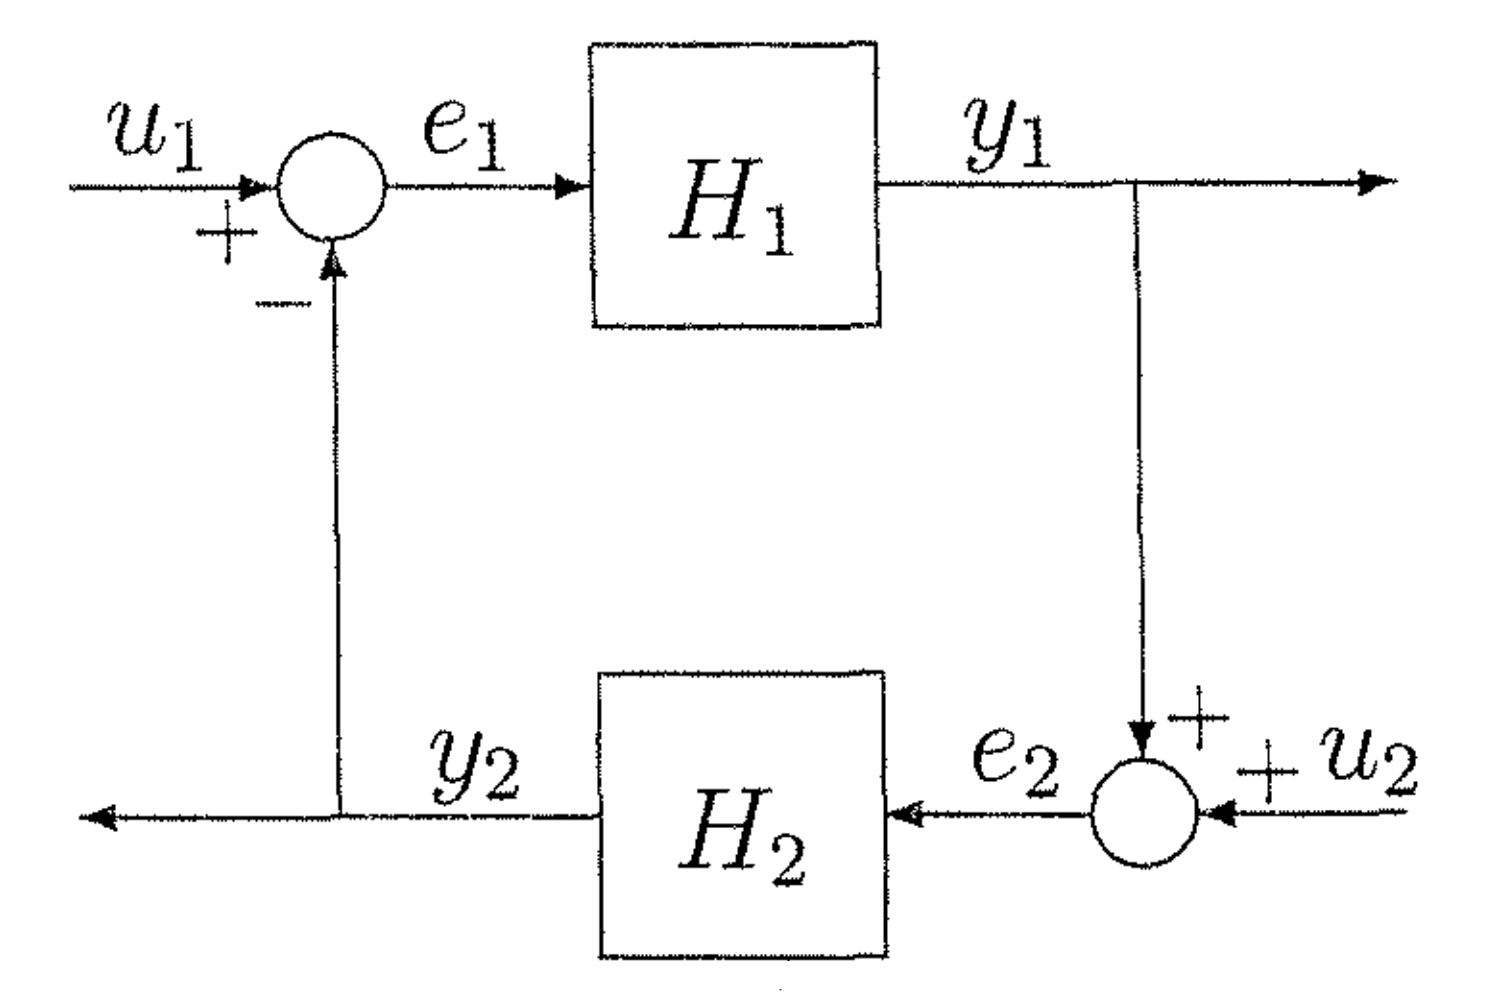
\includegraphics[width=8cm]{feedback-connection.png}
	\caption{Feedback connection}
\end{figure}

\paragraph{Theorem 6.1}
The feedback connection of two passive systems is passive, with $V = V_1 + V_2$.

\paragraph{Theorem 6.2 ($\mathcal{L}_2$-stability of feedback connection)}
If $H_1$ and $H_2$ satisfy
\begin{equation}
	e_i\T y_i \geq \dot{V}_i + \epsilon_i e_i\T e_i + \delta_i y_i\T y_i
\end{equation}
and
\begin{equation}
	\epsilon_1 + \delta_2 > 0 \mbox{ and } \epsilon_2 + \delta_1 > 0
\end{equation}
then the feedback connection is finite-gain $\mathcal{L}_2$-stable.